\documentclass[a4paper,11pt]{article}
\usepackage{graphicx}
\usepackage[utf8]{inputenc}
\usepackage[english]{babel}
\usepackage{url}
\usepackage{natbib}
\usepackage{longtable}
\usepackage[export]{adjustbox} %image adjusting

\usepackage{setspace,caption}
\captionsetup{font=doublespacing}% Double-spaced float captions
\doublespacing% Double-spaced document text
\usepackage{lipsum}
\usepackage{titlesec}
\titleformat{\chapter}{\huge}{\thechapter.}{20pt}{\huge\bf}
\usepackage[margin=1in]{geometry}
\setcitestyle{authoryear,open={(},close={)}}

%Import for Code Style writing. Use \begin{lstlisting]
\usepackage{listings}
\usepackage{color}

\definecolor{dkgreen}{rgb}{0,0.6,0}
\definecolor{gray}{rgb}{0.5,0.5,0.5}
\definecolor{mauve}{rgb}{0.58,0,0.82}

\lstset{frame=tb,
  language=Java,
  aboveskip=2mm,
  belowskip=2mm,
  showstringspaces=false,
  columns=flexible,
  basicstyle={\small\ttfamily},
  numberstyle=\tiny\color{gray},
  keywordstyle=\color{blue},
  commentstyle=\color{dkgreen},
  stringstyle=\color{mauve},
  breaklines=true,
  breakatwhitespace=true,
  tabsize=3
}

%End import

%inputminted -- to import code from file

\renewcommand{\labelenumii}{\theenumii}
\renewcommand{\theenumii}{\theenumi.\arabic{enumii}.} %change listing style to numbers instead of (a,b,c)

\begin{document}
	\title{	\begin{figure}[h]
		\centering
		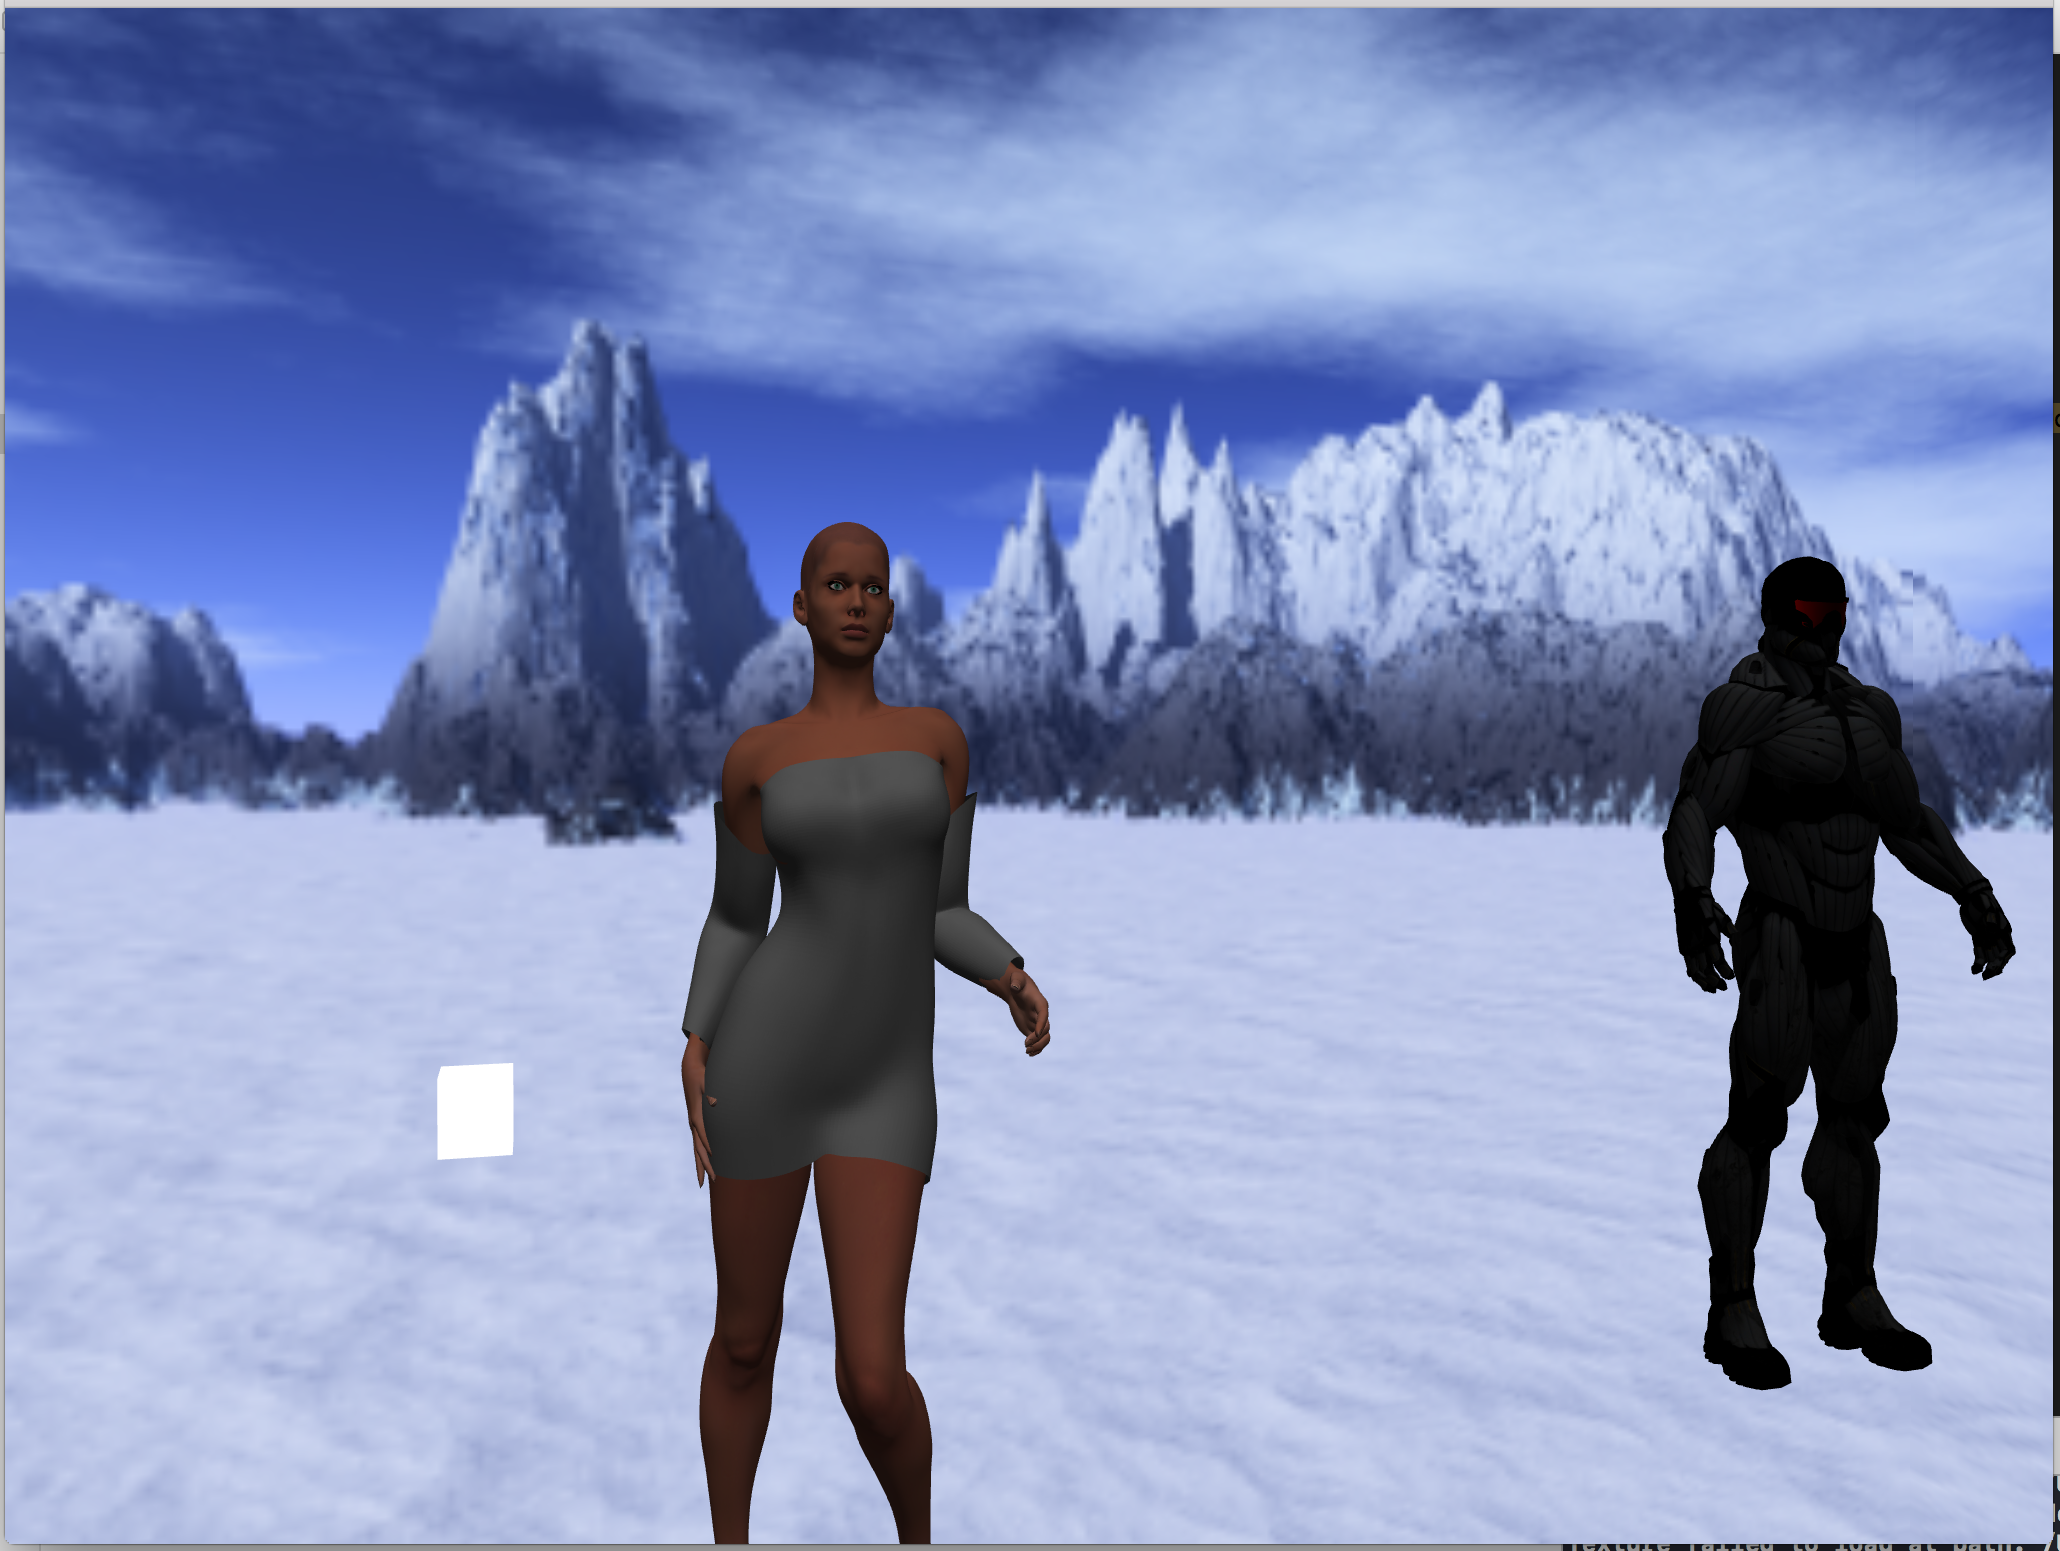
\includegraphics[scale=0.4]{BK}
		\label{HW-logo}
		\vspace{2 cm}
	\end{figure} 
	Graphics Pipeline and Basic Game Engine}
	\author{Rashid Hafez}
	\date{\today}
	\maketitle
	
	\newpage
	\section{Introduction}
	\paragraph{}
		This paper presents a fundamental game engine programmed using the OpenGL API in for C++. I briefly discuss multiple fundamental principles of modern day graphics, such as the graphics pipeline and various rendering techniques. Furthermore I will demonstrate some of the basic functionalities of modern day games, such as camera and animation, along with code samples.
		
	\clearpage
	\newpage
	\section{Class Structure/Abstraction}
		
		The program is broken down into multiple classes (refer to figure \ref{class}). The main class initializes and calls all the other objects, this is also where one would load their models in, given a specific path. This program was created to imitate a very basic fundamental game engine, therefore some aspects must be automated when creating models.
		
		
		\begin{figure}
		\centering
		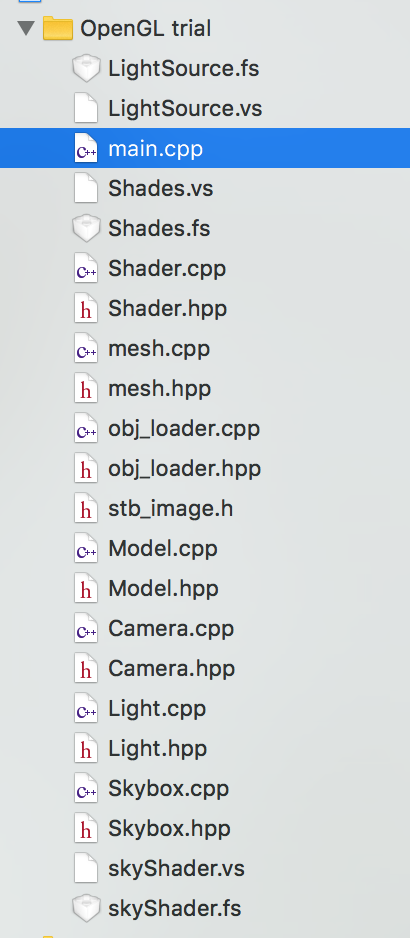
\includegraphics[scale=0.5]{class.png}
		\caption{All the classes in the project}
		\label{class}
		\end{figure}
		
	The following function automates the MVP matrix allocation.
		\begin{lstlisting}
		
	void setCamera(GLuint ID, glm::vec3 translation, float angle, bool trans){
	glm::mat4 projection = glm::perspective(glm::radians(camera.Zoom), (float)width / (float)height, 0.1f, 100.0f);
    
    GLuint proj = glGetUniformLocation(ID, "projection"); //projection IS UNIFORM VARIABLE IN SHADER
    glUniformMatrix4fv(proj, 1, GL_FALSE, &projection[0][0]);
    
    glm::mat4 view = camera.GetViewMatrix();
    GLuint viewI = glGetUniformLocation(ID, "view"); //view IS UNIFORM VARIABLE IN SHADER
    glUniformMatrix4fv(viewI, 1, GL_FALSE, &view[0][0]);
    
    glm::mat4 model(1.0f);
    
    if(trans){
        model = glm::translate(model, translation);
        model = glm::rotate(model, glm::radians(angle), glm::vec3(1.0f, 1.0f, 1.0f));
    }
    else{
        model = glm::mat4(1.0f);
    }
    
    GLuint modelI = glGetUniformLocation(ID, "model"); //model IS UNIFORM VARIABLE IN SHADER
    glUniformMatrix4fv(modelI, 1, GL_FALSE, &model[0][0]);
}

		\end{lstlisting}
	
		
	\section {Shaders}
	
	\paragraph{}
		Shaders are very important, this is one of the classes and functionalities of this engine. The constructor takes in a string file path of where both shaders are. In order for the shader loader to work, you must save both fragment and vertex shader as the same name. In this class we can bind the vertex attributes to tell the shader which location refers to which vertex attribute. 
		
	\begin{figure}
	\centering
	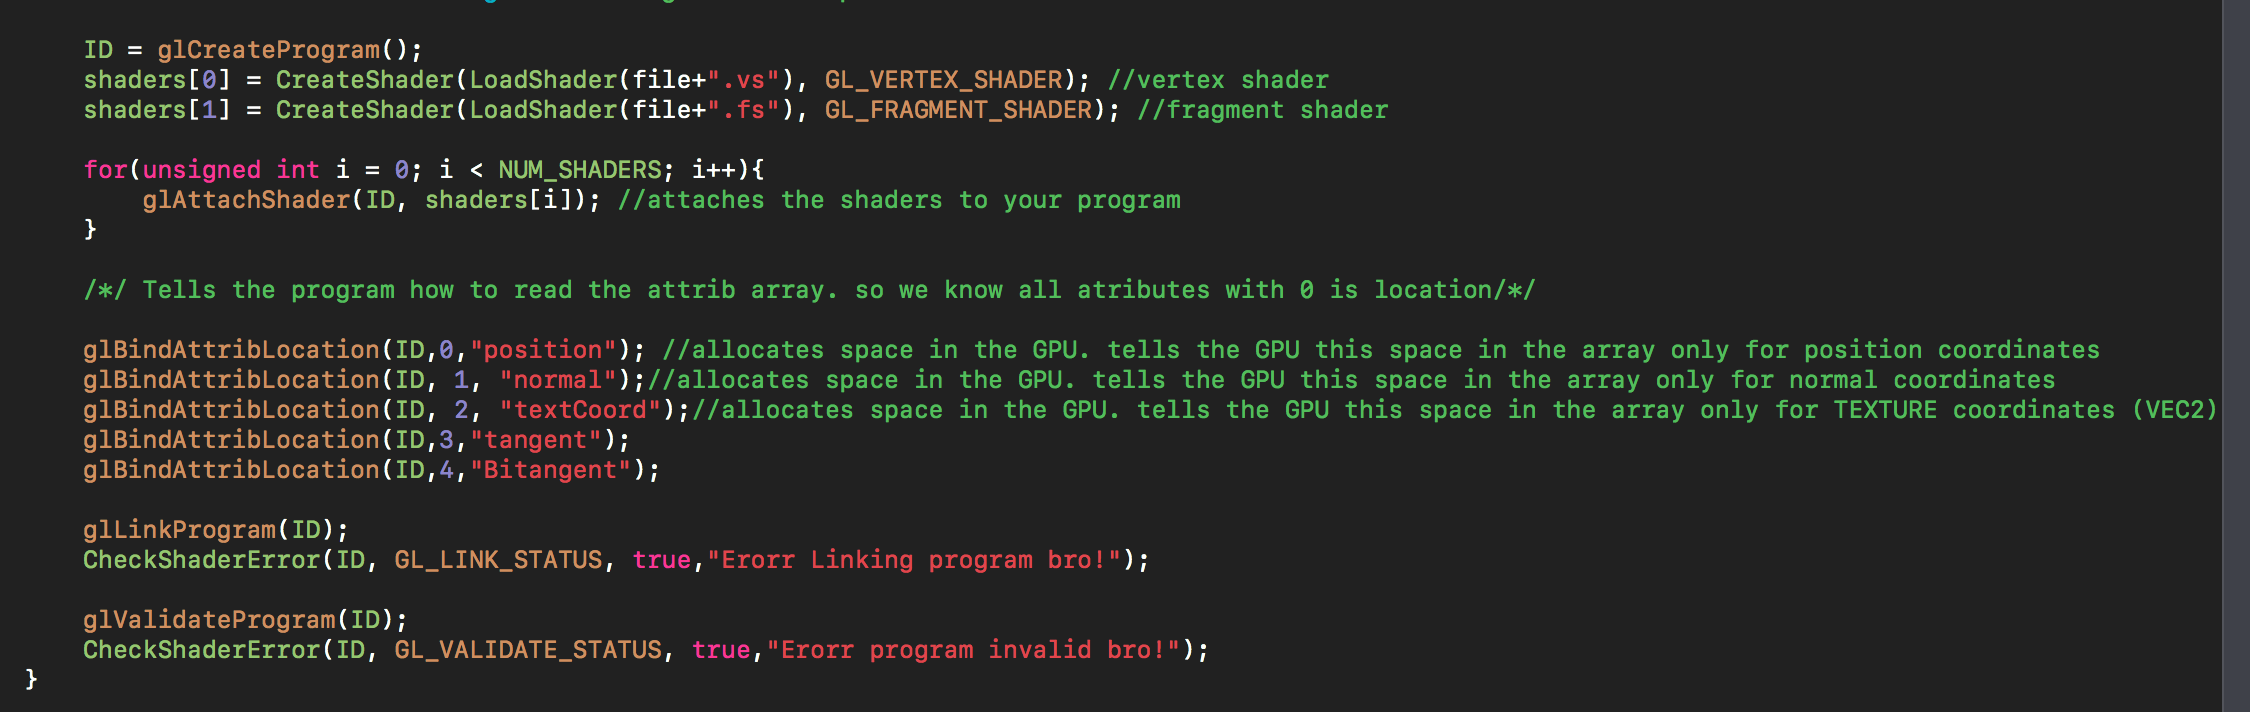
\includegraphics[scale=0.5]{bertex_shader.png}
	\caption{Shader Class file.}
	\label{shaderC}
	\end{figure}
	
	I used 3 different sets of pairs of shaders. 1 pair for the model loading of the human models, 1 pair for the light objects, so that it does not interfere with the normal models and 1 pair for the background/skybox.
	
	The vertex shader sends the fragment position to the fragment shader. When we want to calculate light functions, we send the normal to the fragment shader to calculate the normal, but we want to remove the transfromation properties so we use the following command: 
	
	``vec3 normalT = mat3(transpose(inverse(model))) * vec3(normal.xyz);''
	
	When we want to calculate the position of each fragment we use this function:
	  $gl_Position = projection * view * model * FragPos; //used to be *vec4(position,1.0);$
	  
	  This will draw the position of the fragment according to the MVP matrices set in the main program, since they are UNIFORM they can be read in the shader aswell.
	
	The main shader class contains 2 structs for initializing 2 different lights (see figure \ref{struct})
	
	Then two different functions to calculate how light is rendered from the light source to the object.
	
	For direction light, we use the function called ``TheSun'' takes in the parameters of the struct light.
	
	When calculating directional light we need to calculate how the light hits the object, we calculate the light FROM the source TO the object. Therefore we use this function: 
$vec4 lightDir = normalize(-sun.lightPos);$ //normalize returns a vector with the same direction as its parameter, v, but with length 1."
This function returns the vector of the light direction going towards the object.

For point lights we want the vector to calculate light FROM the object TO the light source. We use this function:

$vec4 lightDir = normalize(plight.position - fragPos); $

For my skybox/cubemap texture:

\begin{lstlisting}
void main()
{
    TexCoords1 = position; //setting the texture as position!
    vec4 pos = projection * view * vec4(position,1.0);
    gl_Position = pos.xyww; //Z COORDINATE ISN'T USED FOR BACKGROUND IMAGES. W is the homogenous coordinate
}
\end{lstlisting}

The skybox doesnt need perspective, therefore we just set the Z coordinate to the homogenous coordinate, for a static background.

\subsection{Animation}

The following code shows how to use keys from the keyboard to influence vectors. This function was added by myself to effect only the point light colour. We change the DIFFUSE vector of the point light, since it is a ``vec3 '' we can associate XYZ with RGB and change these according to what button the user presses.
	
	\begin{lstlisting}
	if(glfwGetKey(window, GLFW_KEY_X) == GLFW_PRESS) {
        if(glfwGetKey(window, GLFW_KEY_R) == GLFW_PRESS) pLightColour.r -= 0.1f;
        if(glfwGetKey(window, GLFW_KEY_G) == GLFW_PRESS) pLightColour.g -= 0.1f;
        if(glfwGetKey(window, GLFW_KEY_B) == GLFW_PRESS) pLightColour.b -= 0.1f;
    }
    else if (glfwGetKey(window, GLFW_KEY_R) == GLFW_PRESS){
        if (glfwGetKey(window, GLFW_KEY_X) != GLFW_PRESS) pLightColour.r += 0.1f;
    }
    else if (glfwGetKey(window, GLFW_KEY_G) == GLFW_PRESS){
        if (glfwGetKey(window, GLFW_KEY_X) != GLFW_PRESS) pLightColour.g += 0.1f;
    }
    else if (glfwGetKey(window, GLFW_KEY_B) == GLFW_PRESS){
        if (glfwGetKey(window, GLFW_KEY_X) != GLFW_PRESS) pLightColour.b += 0.1f;
    }
}
	\end{lstlisting}

	
	Animation of moving light source:
	
	\begin{lstlisting}
	 
        float pX = 10.0f * sin(deltaTime);
        float pY = 15.0f +cos(deltaTime)+10.0f/tan(deltaTime)*sin(deltaTime); //10.0f is the offset
        float pZ = 10.0f * cos(deltaTime);
        pLightPos = glm::vec3(pX,pY,pZ);
        
	\end{lstlisting}
	
	pLightPos is then updated in the Position light struct, the vector position is assigned the values of the pLightPos vector. The SIN AND COS AND TAN give the object its smooth rotational values and angles. The above code snippet must be executed in the loop.
	
	
	
	
\begin{figure}
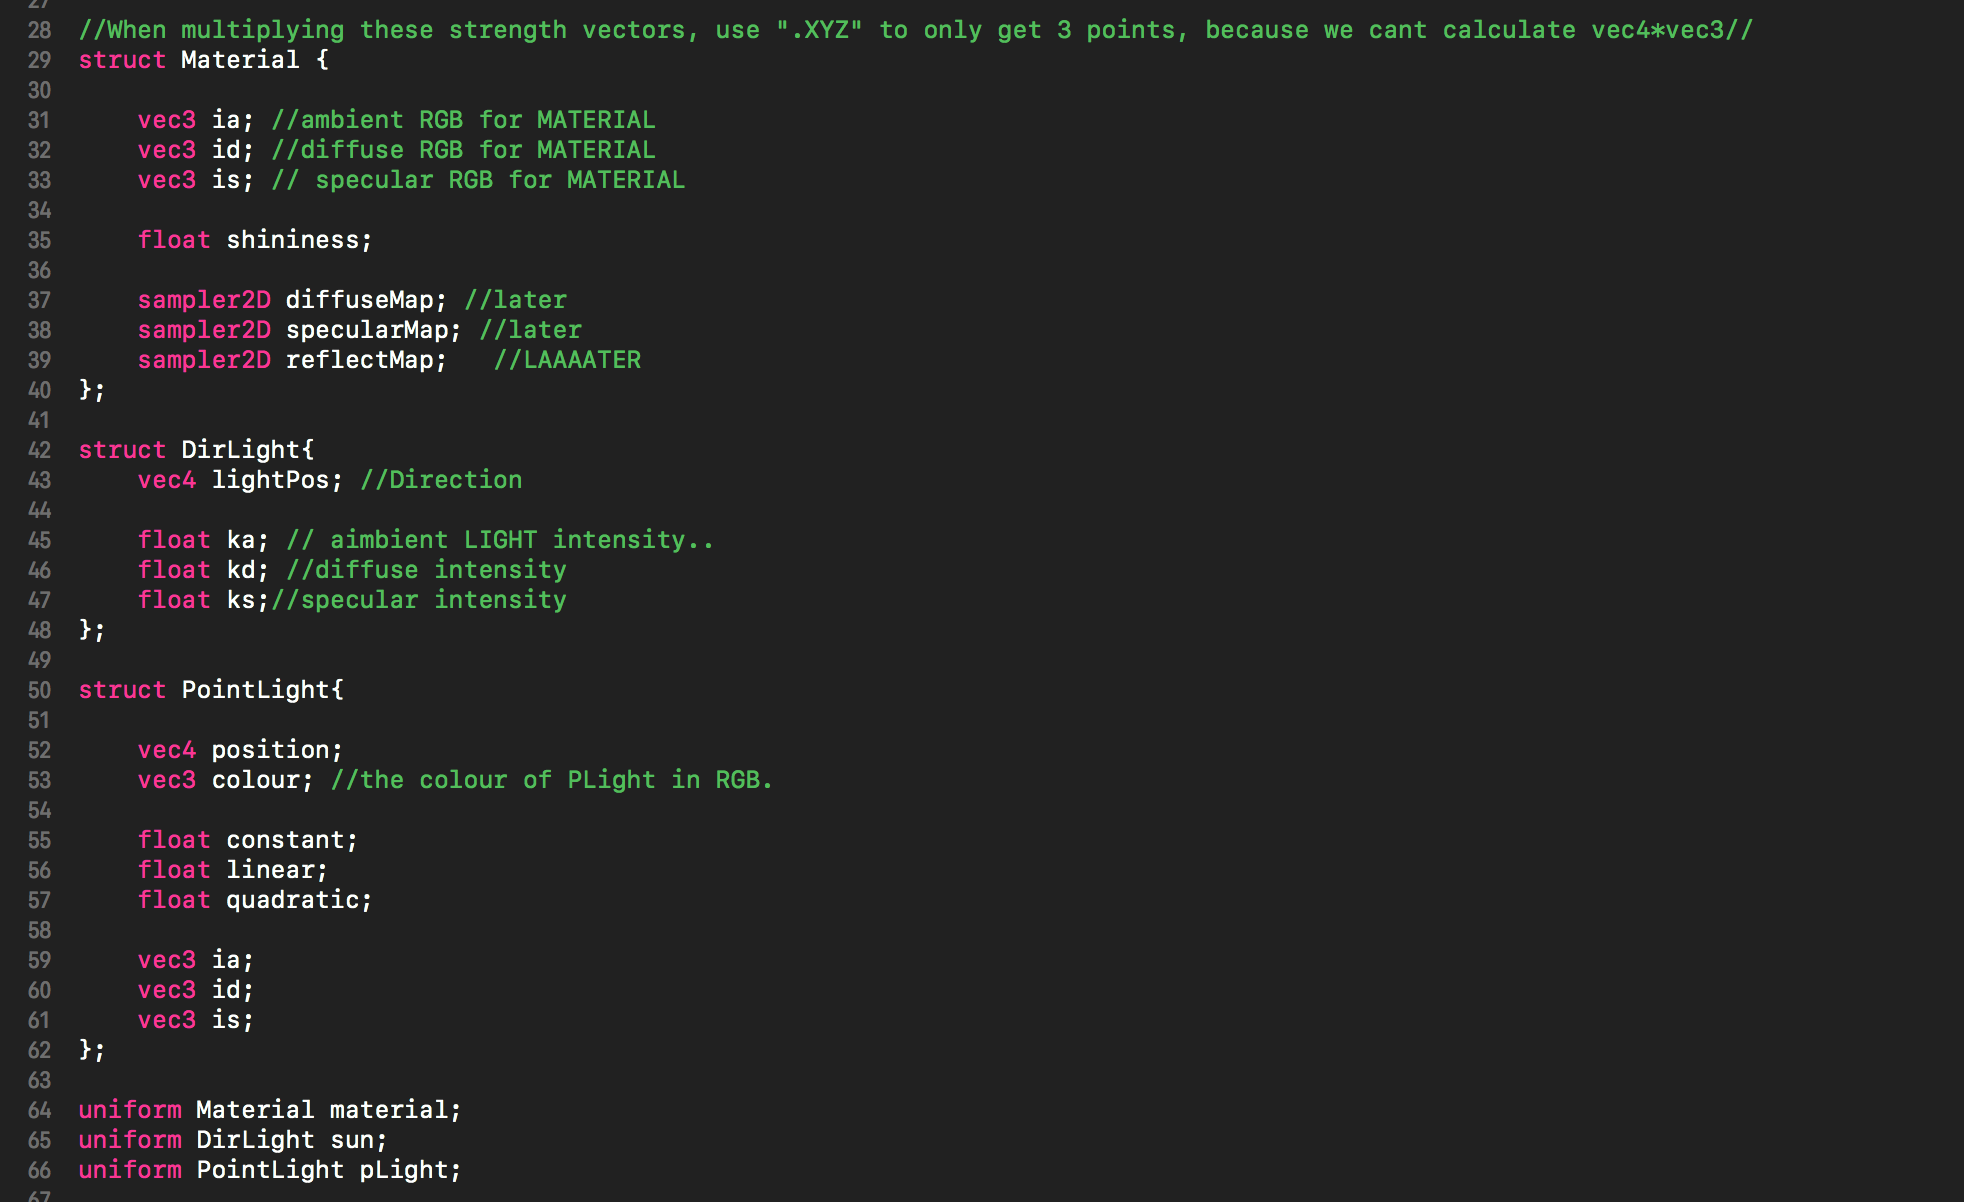
\includegraphics[scale=0.5]{struct.png}
\caption{Snippet demonstrating structs inside shader.}
\label{struct}
\end{figure}
\clearpage
\newpage

	\section{Model Loading}
	
	Model loading is constructed of multiple elements. Firstly, I used an open source external add on for blender which can automate human model creation (MANUELBASTIONILAB(2018)). Then I added and created the clothes objects myself.
	 
	 Secondly in the program code, I used an open source external library (ASSIMP 2018), to read object files and store the object in a data structure scene, consisting of tree nodes for each model and each object of the model.

\begin{figure}
\centering
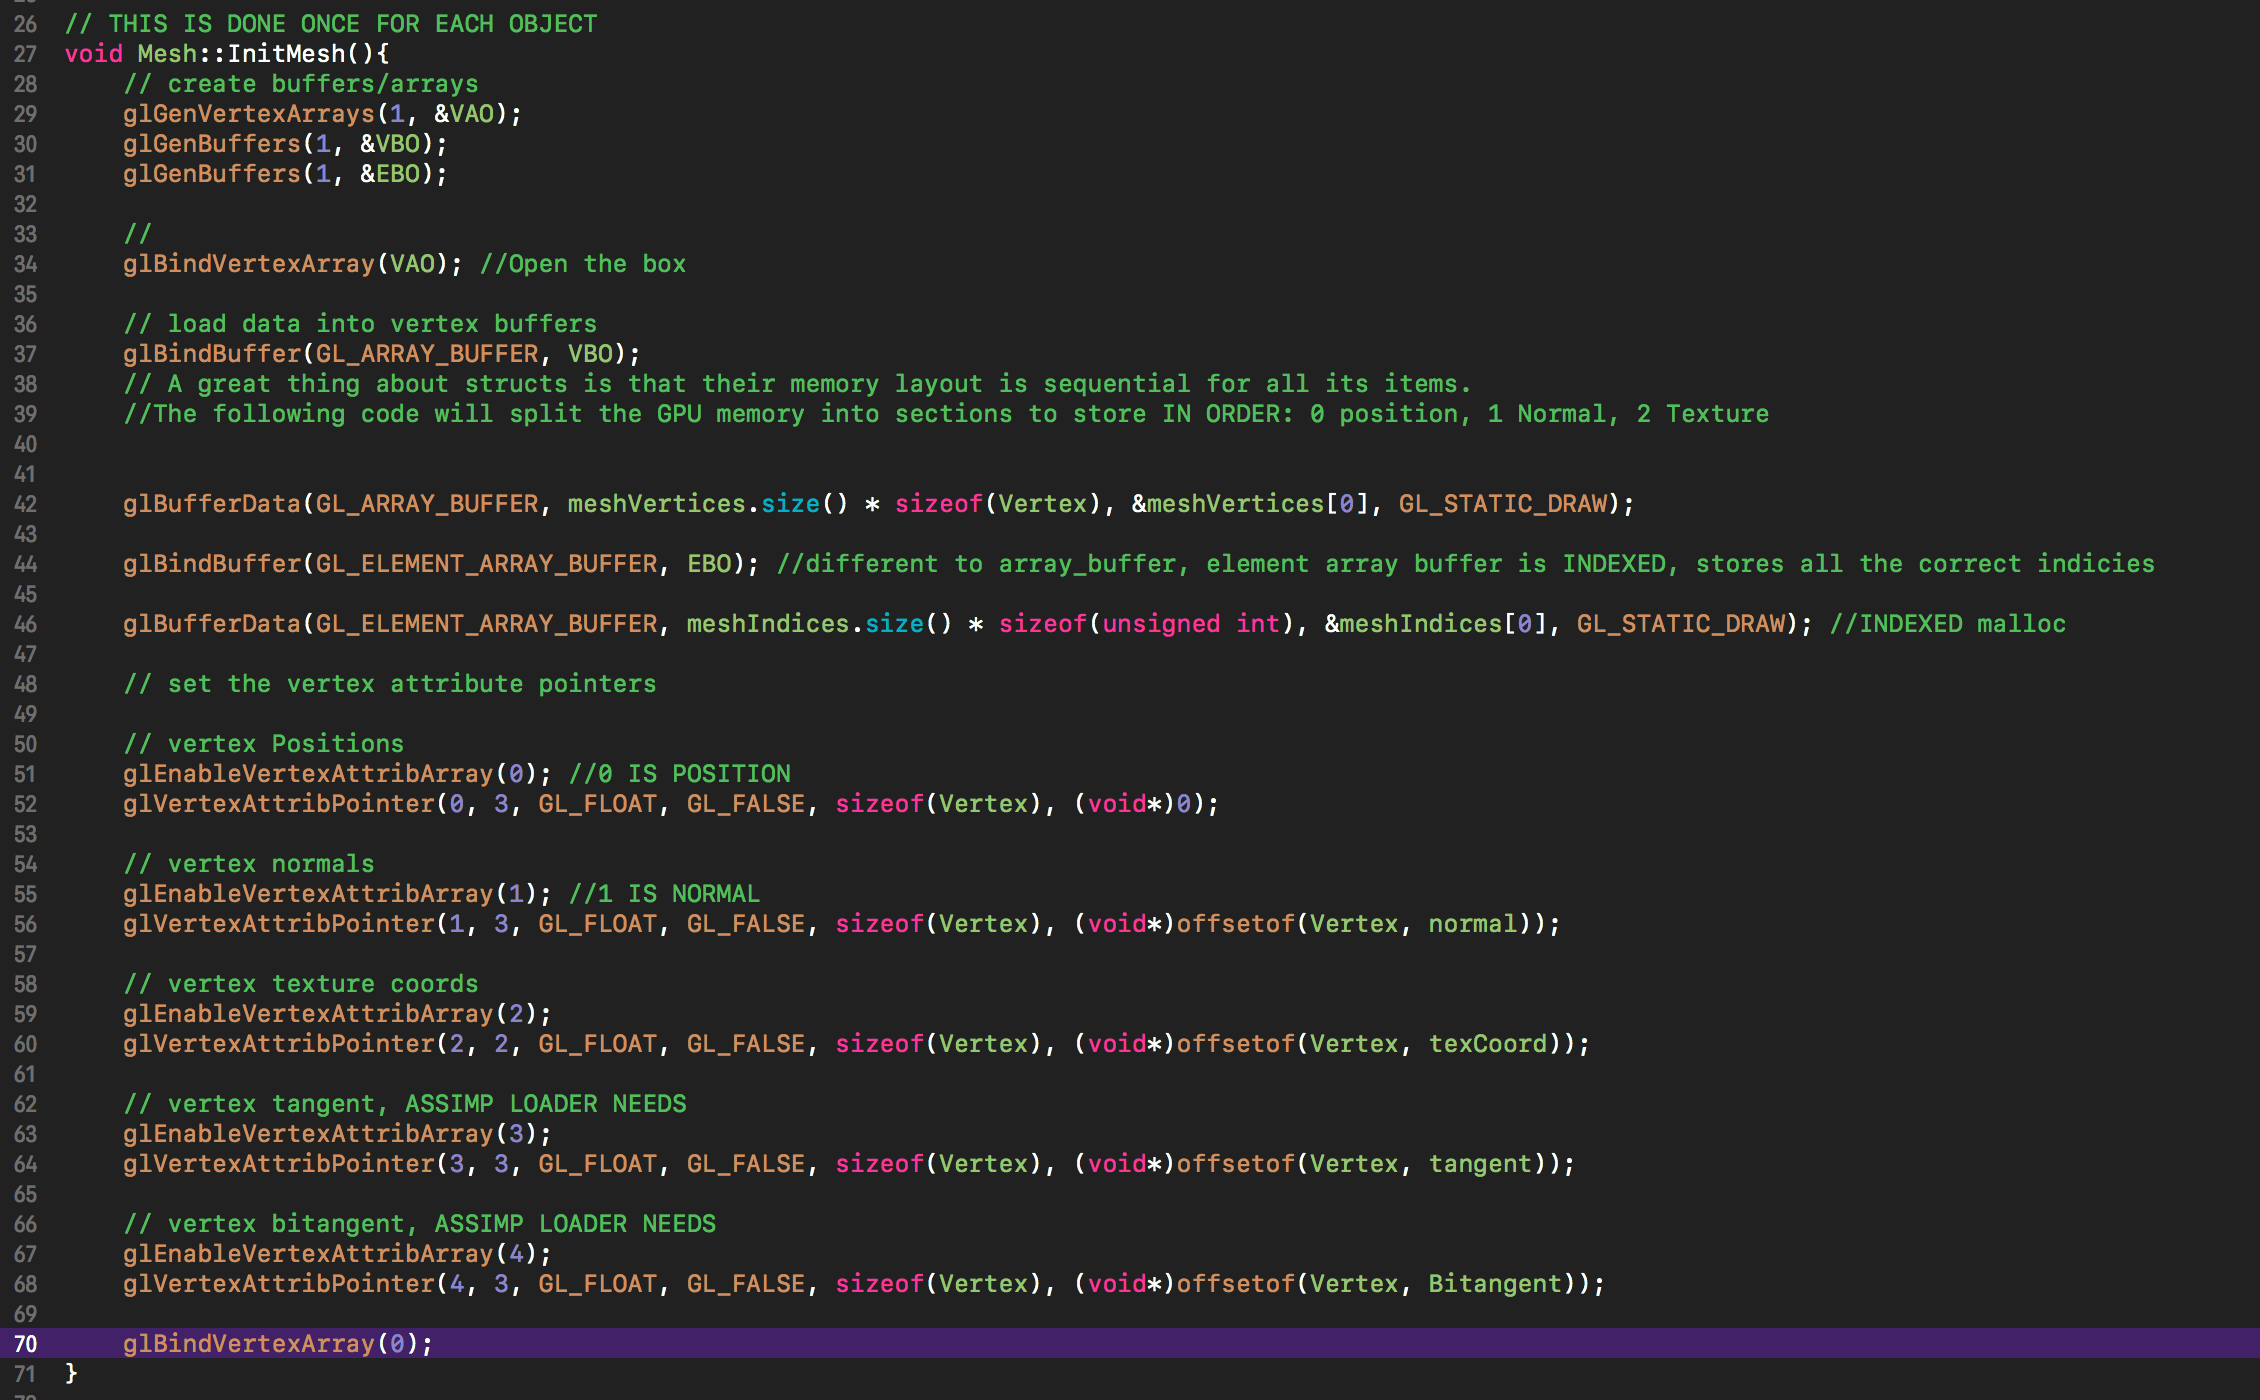
\includegraphics[scale=0.5]{VAO.png}
\caption{Snippet showing allocation of buffers and vertex array objects.}
\label{VAO}
\end{figure}


\section{References}

	\begin{enumerate}
		
		\item Model MANUELBASTIONILAB 2018:  http://www.manuelbastioni.com/manuellab.php
		
		\item Model Loader ASSIMP 2018: http://www.assimp.org/
							
		\end{enumerate}


\end{document}
